\section{Methodology}
This section should outline the approach and methods you will use to achieve the project objectives. It should include the following subsections:

\subsection{Requirement identification}
Conduct a thorough review of existing systems, solutions, or academic literature related to your project. 
\begin{figure}[h]
    \centering
    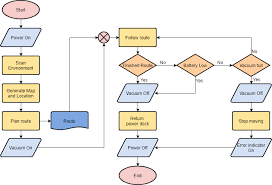
\includegraphics[width=0.5\linewidth]{Images/flow.png}
    \caption{Caption}
    \label{fig:enter-label}
\end{figure}
Discuss how previous work relates to your project and identify any limitations or gaps that your project aims to address.

\subsubsection{Study of Existing System / Literature Review}
Summarize your research on existing solutions, systems, or literature related to your project. Discuss their strengths, limitations, and how your project will build upon or differ from them.

\subsubsection{Requirement Analysis}
Identify and analyze your project's specific requirements, constraints, and assumptions. This includes technical, operational, and user requirements.

\subsection{Functional Requirement}
Add a table consisting the list of features the software will provide (e.g., user registration, reporting, data analytics) and specific use case scenarios.
\subsection{Non-Functional Requirement}
Add a table listing the non-functional requirement of the system (e.g., Performance, Scalability, Security, Usability, Reliability).

\subsection{Feasibility Study}
\subsubsection{Technical}
 Assess the technical feasibility of your project, including the availability of necessary resources, tools, and expertise.

Assess the technical resources and expertise required for the project. Discuss whether the project is technically feasible, considering the availability of technology, tools, and skills.
 
\subsubsection{Operational}
Evaluate the operational feasibility, considering factors such as user acceptance, organizational support, and compatibility with existing systems.

Evaluate whether the project can be successfully implemented and used within the intended environment. Discuss any operational challenges and how they will be addressed.

\subsubsection{Economic}
 Conduct a cost-benefit analysis to determine the economic feasibility of your project. Consider factors such as development costs, maintenance costs, and potential benefits or savings.

\begin{table}[h]
    \centering
    \caption{sample Cost-Benefit Analysis of the Proposed Project}
    \begin{tabular}{@{}llcc@{}}
        \toprule
        \textbf{Item} & \textbf{Description} & \textbf{Cost (\$)} & \textbf{Benefit (\$)} \\ \midrule
        Development Costs & Software Development & 15,000 & - \\
        Hardware Costs & Servers and Equipment & 5,000 & - \\
        Training Costs & User Training Sessions & 2,000 & - \\
        Maintenance Costs & Annual Maintenance & 1,000 & - \\
        \midrule
        \textbf{Total Costs} &  & \textbf{23,000} & - \\ \midrule
        Increased Efficiency & Time Savings & - & 30,000 \\
        Improved User Satisfaction & User Feedback & - & 10,000 \\
        Revenue Increase & New Customers & - & 20,000 \\
        \midrule
        \textbf{Total Benefits} &  & - & \textbf{60,000} \\ \midrule
        \textbf{Net Benefit} &  & \textbf{23,000} & \textbf{37,000} \\ 
        \bottomrule
    \end{tabular}
    \label{tab:cost-benefit}
\end{table}

 Analyze the cost-effectiveness of the project. Consider the budget, expected benefits, and potential return on investment. Provide a cost-benefit analysis to justify the project's financial viability.
 
\subsubsection{Schedule(Gantt chart showing the project timeline)}
 Include a Gantt chart or timeline that outlines the key milestones, tasks, and dependencies for your project. This will help demonstrate the feasibility and planning of your project. Typically we are bounded by 10-12 weeks.
 
\begin{figure}[H]
    \centering
    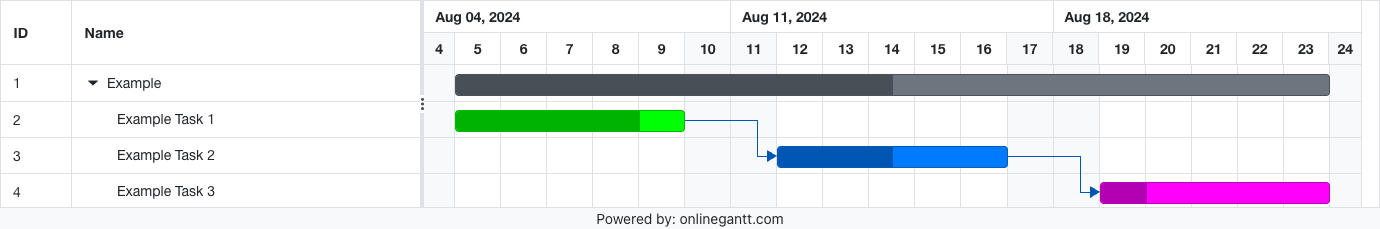
\includegraphics[width=1\linewidth]{Images/gantt.png}
    \caption{Sample Gantt Chart demonstrating schedule feasibility}
    \label{fig:enter-label}
\end{figure}

Include a Gantt chart or timeline that outlines the key milestones, tasks, and dependencies for your project. This will help demonstrate the feasibility and planning of your project. Maybe we can use \url{https://www.onlinegantt.com/#/gantt} to create a Gantt chart as per our need.
  
\subsection{High-Level Design of System}
Provide an overview of the proposed system's architecture and design. This should include:

\subsubsection{Methodology of the proposed system}
Methodology of the Proposed System: Describe the overall approach and techniques that will be used to develop the system. Design May be Structured or Object Oriented as per the approach followed.

\subsubsection{Flow Charts/Working Mechanism of Proposed System}
Include flowcharts or diagrams that illustrate how the system will function.

\begin{figure}[H]
    \centering
    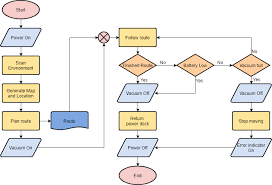
\includegraphics[width=0.5\linewidth]{Images/flow.png}
    \caption{Sample flowchart}
    \label{fig:enter-label}
\end{figure}

We may use online tools like \url{https://app.diagrams.net/} or \url{https://www.figma.com/} to create such diagrams but are not limited to.

\subsubsection{Description of Algorithms}
Explain any algorithms that will be implemented, detailing their purpose and how they contribute to solving the problem. This is mandatory.